%%Methodology
%% methodology Intro

To address the central inquiry of this research – ``How do users respond to complex facades crafted with digital fabrication, as assessed through virtual reality, and how does this insight shape forthcoming architectural trends?'' – the methodology unfolds in three distinct sections: Image Complexity Analysis, VR Building Complexity System Development, and Experiment Design.
And the workflow is illustrated in Figure\ref{fig:MethodologyFlowchart}.

The first component, Computational Image complexity analysis (CICA) involves the development of a Python script tailored to process images systematically, yielding complexity scores that quantitatively gauge the intricacy of architectural designs.
This component serves a dual purpose: corroborating the theoretical architectural style analyses established on the theory framework section and also as an initial framework to rank a series of facades designs to be used on the VR system to compare participants perceptions in an experiment mimicking various complexity levels in building facades.

The second component, VR Building Complexity System Development, revolves around the creation of a Virtual Reality (VR) system designed to immerse users within a building environment.
Within this virtual realm, users possess the capability to manipulate facade complexity across ten discrete levels, a hierarchy determined by the Computational Image Complexity Analysis module's prior rankings.

In the third section, the experiment design determines the method used to evaluate the level of complexity that users of a building would accept through the use of Virtual reality simulation using a Heads-up Display (HUD).
Following a similar approach to previous studies using VR assessment\cite{Wolfartsberger2019}, a group of participants was invited to engage in an experiment to measure Building Complexity perception across three distinct stages: The ``VR interaction stage'', the ``Screen based Image ranking stage'' and the ``Post-interaction survey'' stage.
No prior experience in facade design was required from participants.

The experiment and overall framework to get the results to validate the hypothesis will be developed on this section

%% Figure Methodology flowchart
    \begin{figure}[!htb]
      \centering
      % trim=left 190 down 250 right 150 top5
      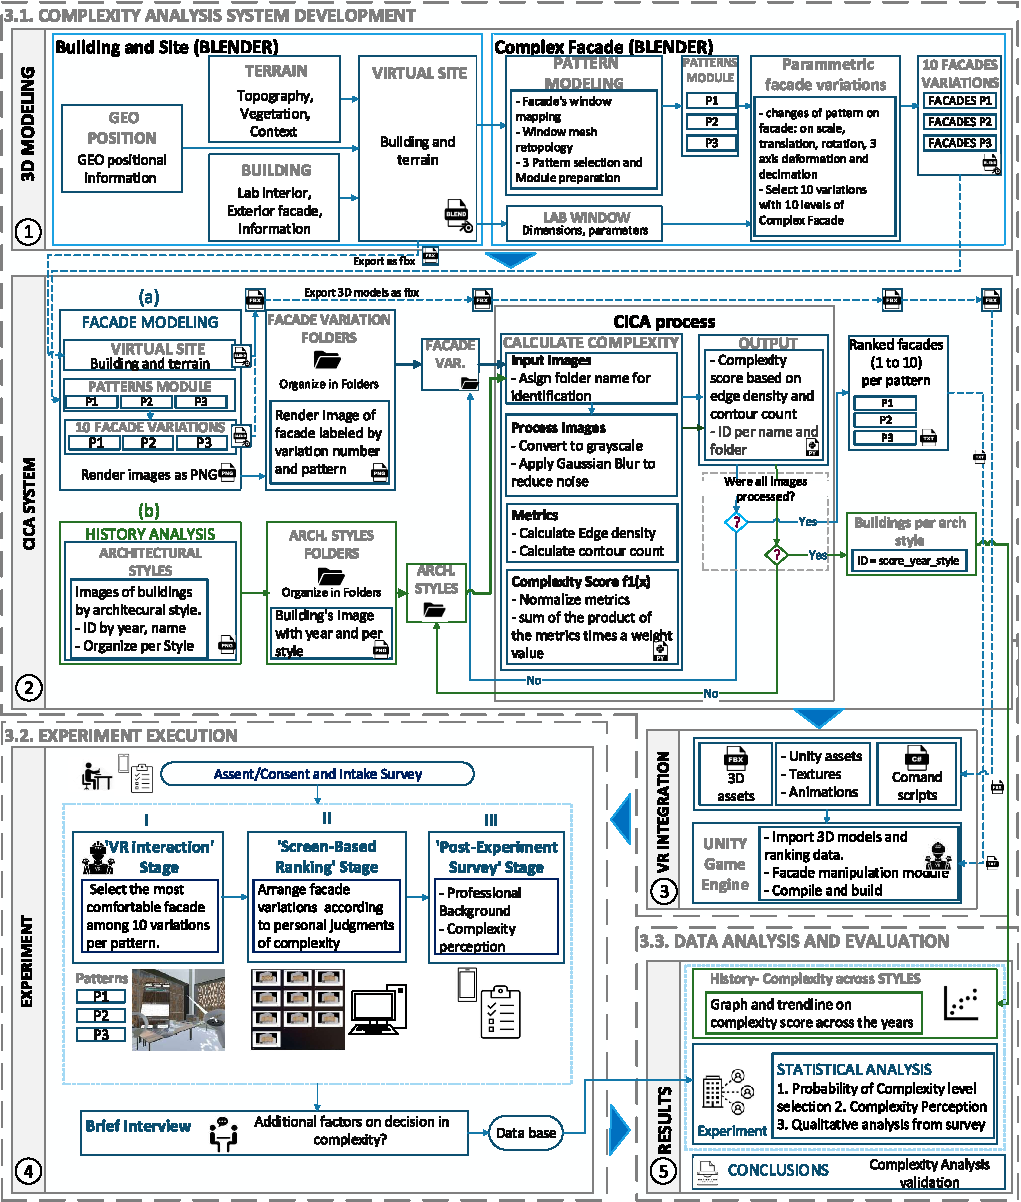
\includegraphics[width= \linewidth, trim=0 0 0 0, clip]{Images/MethodologyFlowchart}
      \caption{Methodology flowchart}
      \label{fig:MethodologyFlowchart}
    \end{figure}